\documentclass[9pt,twocolumn,twoside]{styles/osajnl}
\usepackage{fancyvrb}
\journal{i524} 

\title{Predicting Readmission of Diabetic patients}

\author[1,*]{Kumar Satyam}
\author[1,**]{Piyush Shinde}
\author[1,***]{Srikanth Ramanam}

\affil[1]{School of Informatics and Computing, Bloomington, IN 47408, U.S.A.}

\affil[*]{Corresponding authors: ksatyam@indiana.edu}
\affil[**]{Corresponding authors: pshinde@iu.edu}
\affil[***]{Corresponding authors: srikrama@iu.edu}

\dates{project-000, \today}

\ociscodes{Hadoop, Spark, Ansible, Python}

% replace this with your url in github/gitlab
\doi{\url{https://github.com/cloudmesh/classes/blob/master/project/S17-IR-P004/report/report.pdf}}


\begin{abstract}
We are trying to predict whether a diabetic patient will be readmitted to the hospital, using several features representing patient and hospital outcomes. We will use Hadoop/Spark distributed architecture on multiple clouds as the core infrastructure and machine learning classification algorithms for data analysis.
\newline
\end{abstract}

\setboolean{displaycopyright}{true}

\begin{document}

\maketitle

\tableofcontents % Print the contents section

\section{Introduction}

We will use Hadoop to split the dataset and transfer the data chunks to different data nodes. We will use Ansible to install pre-requisite softwares and push configurations on different machines. The data chunks would then be analyzed using machine learning techniques and the results would be aggregated predicting whether a patient would be readmitted or not. This information would help hospitals to be better prepared for readmitting patients.


\begin{figure}[h]
    \centering
    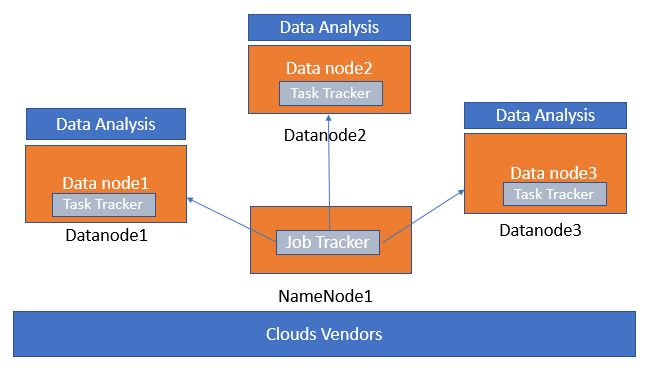
\includegraphics[scale=0.57]{images/1}
    \centering
    \caption{Deployment Architecture}
    \end{figure}

\section{Timeline}

\begin{center}
\begin{tabular}{ c l } 
 \hline
Week & Target \\
\hline
1 & Finalizing Technologies, Data Cleansing \\
2 & Hadoop/Spark Deployment on Chameleon Cloud \\ 
3 & Troubleshooting\\ 
4 & Data Analysis \\ 
5 & Deployment on other cloud using Ansible\\ 
6 & Benchmarking  \\ 
7 & Report Preparation \\ 
 \hline
\end{tabular}
\end{center}



\section{Technologies}
\begin{center}
 \begin{tabular}{l l} 
 \hline
 \textit{Technology} & \textit{Usage}  \\  
 \hline 
 \textbf{Hadoop}\cite{www-hadoop}/\textbf{Spark} \cite{www-spark} & Distributed Data Storage  \\
 \hline
 \textbf{Python}\cite{www-python}/\textbf{Java}\cite{www-java}/\textbf{Scala}\cite{www-scala} & Development \\
 \hline
 \textbf{Ansible} \cite{www-ansible} & Application Deployment \\ & $\&$ Configuration Management \\
 \hline
 TBD & Benchmarking \\
 \hline
 \textbf{LaTex} \cite{www-latex} & Document Preparation \\
 \hline
\end{tabular}
\end{center}
    
\section{Deployment}
We will deploy a master $\&$ multiple slave nodes in the Hadoop/Spark distributed cluster environment. 

We will use \textbf{Ansible} as an automated application and configuration deployment tool. This will enable us to install softwares and push configurations simultaneously from master node to the respective target nodes. 

\section{Benchmarking}
We will assess the performance of the Hadoop/Spark clusters deployed on different clouds. The parameters for benchmarking would be memory usage, storage size and IO throughput.

    
    
\section{Results}
Results of data analysis and benchmarking will be showcased in this section.

\section{Conclusion}
Using the 130-US hospitals dataset \cite{www-dataset} for years 1999-2008, we should be able to analyze factors pertaining to readmission of patients with diabetes. 

\section{Acknowledgments}
This project was a part of the Big Data Software and Projects (INFO-I524) course. We would like to thank Professor Gregor von Laszewski and the associate instructors for their help and support during the course. 

\bibliography{references}

\end{document}
